\section{Gleanings about the Field of Pearls}

I have been reading \emph{The Way of a Pilgrim}, recently, which is a Russian peasant's account of his discovery of the prayer of the heart. The anonymous author had lost his father and wife to an illness, and been dispossessed by a worthless brother, who had also crippled him when they were younger. Henceforth, the man becomes a beggar, and then, after hearing in Church St. Paul's admonition to ``pray without ceasing", a pilgrim to discover what the inner or hidden meaning of this was.

\begin{wrapfigure}{rt}{.3\textwidth}
 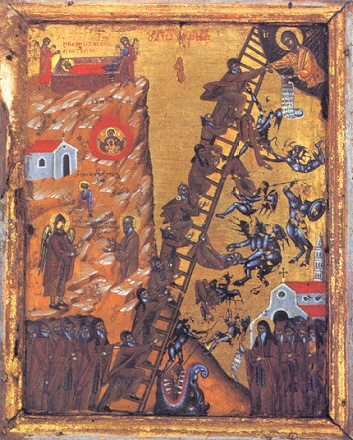
\includegraphics[scale=.6]{a20130621GleaningsabouttheFieldofPearls-img001.jpg}
\end{wrapfigure}

Somehow, he obtains a copy of the \emph{Philokalia}, and literally learns it by heart from reading it every day. Additionally, his old \emph{starets} sometimes appears to him in a dream, and offers him guidance, not only spiritual but even to face physical challenges, such as curing an old woman who has been kind to the pilgrim.

\begin{quotex}
``It costs nothing but the effort to sink down in silence into the depths of one's heart and call more and more upon the radiant name of Jesus. Everyone who does that feels at once the inward light, everything becomes understandable to him, he even catches sight in this light of some of the mysteries of the kingdom of God. And what depth and light there is in the mystery of a man coming to know that he has this power to plumb the depths of his own being, to see himself from within, to find delight in self-knowledge, to take pity on himself and shed tears of gladness over his fall and his spoiled will!"

\end{quotex}
It should be instantly apparent to the unbiased reader (whomever they may desire to appear to themselves) that here we have no ``life-denying" or purely passive ``asceticism. On the contrary, this is spoken of as an active power corresponding to the alchemical stage of \emph{rubedo}. You see that they are spoken of as ``tears of gladness``.

There is no doubt that ``Semitic" spirituality in a purely ``exoteric" sense has included many ``life-denying" elements in propagating what appeared to it to be truths. However, we need to make a point that the division exoteric-esoteric is itself part of the problem (as Cologero has alluded to). It is to think in terms of division, separation. Well, this is the problem to begin with! Because ``esotericism" departs (or is corrupted), the ``exoteric" shell attempts to preserve ``Christendom" inside of formulations from which Life has departed. Likewise, esotericism without exoteric landmarks can be dark paths indeed. The thing is to unite the two! \emph{Or, rather, to see that they are already One}.

The pilgrim refers to the Almighty as the ``\emph{merciful and man-loving God}``. This will be too ``materialistic" or even ``humanistic" for Gnostics, just as the Virgin Mary has always scandalized certain highly spiritual individuals (St. Francis designed the manger creche to confound them).

\emph{``Everyone does what he can, as he sees his own path, with the thought that God himself shows the way of his salvation."} This will be not rigid enough for the Pharisees in Christendom, who wish everything to be ``made clear".

\emph{``The mysterious sighing of creation, the innate aspiration of every soul toward God, that is exactly what interior prayer is. There is no need to learn it, it is innate in every one of us."} This will irritate the Protestants (who hate Nature) \& those who wish (like General Namaan) for mightier tasks than bathing in the Jordan to cure their leprosy.

The volume is not the work of a saint or scholar, but a peasant, who comes to know God through ``the Jesus prayer" of hesychasm (which interestingly enough, receives various emphasis or stresses on its syllables, according to the inner spiritual gift of the person praying the prayer). The \emph{starets} comes to him in a dream, and even points out which portions of the\emph{ Philokalia} to read first, and in what order.

As we wander through the desert of Modernity, a pithy man \footnote{\url{http://www.gornahoor.net/?p=6491}} points out that even in God's ``separation" from the modern world, the spiritual man ought to begin to learn to discern signs of His presence, for He can never be finally absent. No decayed corpus of Christendom can prove the lack of His, the Lord's, power. No collapse of the West can prove that, after all, God is mocked. The Supreme Lord will not be mocked, no matter how large scale the rebellion is, nor does His mercy fail even in the dark.

I think a reader here recommended (for which I thank him) \emph{The Three Conversions of the Spiritual Life}, by Garrigou-Lagrange, OP, which my wife bought me for father's day. There is little doubt that out of the ``wreckage" we can salvage, not merely ``much", or even ``all" that we need, but abundantly more so. God has littered the landscape with many treasures, and books such as these testify to an inner heart of Christianity which has existed even during the seemingly dead days of being buried under ground. In fact, since the heart is alive, the body remains as well – not the body the Pharisees promulgate, but the body of the Lord. For instance, Garrigou-Lagrange distinguishes, in direct and explicit parallel to Dionysius' tradition, the three inner stages of purgation, illumination, and union, and what happens when one gets stuck along the way, in between one of the stages. Are any readers here stuck in a spiritual stage they do not understand? He goes on to explain that God the All-Merciful converts a man where he is at. This, by the way, is why the conversion begins in the senses, and doesn't include the soul or spirit to begin with: God isn't going to make someone enlightened against their will! He begins with the beginning stage. When they are purged as to senses, then a purgation of the soul commences, but is ``illuminated" in this more difficult stage: the person now loves not only with the heart, but with strength. The last conversion is a movement into spirit, in which God is loved with the ``soul" (spirit), and finally attains intellectual and perfect and near-continuous (at least) union with God.

As one can see, this involves a ``taking up" of each lower part into a higher part, along with a move of consciousness to the higher plane. From the ``sensual" plane, soul and spirit are one. Only from the soul plane does one even begin to intuit that there are higher regions still. And what comes after this? The Self Beyond the Self?

Look about you, if not in your tradition, then some tradition fit for you. Seek it, and find it: you will seek what you find anyway. It is ultimately not a concept or even an ``ideal" (although it certainly will make use of both along the way), but a path which you already know, as the Russian peasant pilgrim already knew, when he set out on his journey, that he would find his Lord.

By the way, if you have fallen, a repentance equal or greater in fervor than the sin which was committed will re-instate your ``talents" and place you back upon the Ladder. The thing is to climb.



\flrightit{Posted on 2013-06-21 by Logres }

\begin{center}* * *\end{center}

\begin{footnotesize}\begin{sffamily}



\texttt{Jason-Adam on 2013-06-22 at 11:15 said: }

Logres do you think there is a difference between the western spirituality of a Gerrigou-Lagrange and the eastern hesychasts ? I want to resolve for myself once and for all whether Christian spirituality is one, uniting west and east, or if the culturual divide between western Christianity and the eastern church is too great akin to say Christianity and Hinduism.


\hfill

\texttt{Scardanelli on 2013-06-22 at 11:35 said: }

For more on the three stages of spiritual path from the Orthodox perspective, there is an excellent series by Archimandrite Zacharius: The Enlargement of the Heart, The Hidden Man of the Heart, and Remember Thy First Love. I've only begun reading the first, but in skimming through all of them they seem quite good.


\hfill

\texttt{Scardanelli on 2013-06-22 at 11:40 said: }

…And you're a lucky man Logres. All I got for Father's Day was a shirt and tie.


\hfill

\texttt{Logres on 2013-06-22 at 22:55 said: }

Scardanelli, thank you for those recommendations; a huge part of what we are to be about (at this stage) is sharing interests and reading lists – things that would be normative under different conditions. I think it was Jason-Adam who recommended Lagrange, and I am pleased to have read it. I thank you in advance, as I am sure you have steered me well!

Jason-Adam: I have given a lot of restless and restful thought to this, and with the provisio that I defer to any one with higher knowledge, I am bound to say (especially after leafing through Scupoli and reading Lagrange, as well as what I remember from Thomas Merton's commentaries and excerpts on John of the Cross) that the Catholic mystical tradition is substantially identical to what one would find in Orthodoxy. Even making allowances for Romanides' criticisms (and you won't find any stronger critic, unless it was Athanasios Bailey's website @ Orchid Land Publications (now defunct, on the web, although you may be able to dredge archives), the mystical theology of both teach the same truth. I think it might help you to experientially realize that (like Iamblichus and Plotinus, in a way) there is a common ``source" (even though it can't be perceived mentally, it can be intuited, although someone who had attained mystical Union would be able to perceive it mentally, as this is the last stage). If you are a warrior, then your recognition of this commonality will be tempered by a healthy preference for one or the other, and a suspicion for the other, although even this should not keep you from affirming certain elements. Christianity is a ``warrior religion" in many ways: the Vedic side is carefully hidden, whether deliberately or not, \& so like Islam (but to a much lesser extent) Christianity has been a marching and embattled faith, which tends to draw strong lines. You can see the Orthodox fall into a perspective of embattled and reactionary thought, at times, when they begin to denigrate everything Western, because it is ``Western". While this may be a good attitude and stance at times and places (and the warriors will help decide when this is), it cannot be the final word. Even an Orthodox theologian like Evdokimov goes so far as to suggest that there are undiscovered sacraments which God's grace has yet to reveal. since it is infinite. Perhaps one of them will be the reunion of the Church, who knows? That is why it's a blessing to be alive right now. Some of this is sketched in the ``Church of John", ``Church of Peter", ``Church of Paul" outline given by Tomberg and others. Meanwhile, Meanwhile, it's no shame and a great help to ``wake up" to the various dangers and departures within the Tradition – my guess is that Orthodoxy has many of its own. The Church is indefectible, not perfect.


\hfill

\texttt{Jason-Adam on 2013-06-24 at 13:00 said: }

@ Logres, I agree with you that essential Catholic and Orthodox mysticism takes you to the same place while using different language, which is why I do not agree with the Orthodox minds of a Romanides or a Dugin who see only evil in the Western church. My approach to spirituality is indeed affected by my warrior calling, which causes me to be partial to my own ancestors and heritage and as such I just find myself not fitting in with non-Western forms, even though I do admire from afar those forms. When it comes to relations between the churches, I accept Soloviev's two lung thesis from Russia \& the Universal Church which is why I oppose deeply people like Dugin who try to widen the schism between east and west and also those westerners who think being traditional means hating yourself, your family and your culture.


\hfill

\texttt{Logres on 2013-06-24 at 14:52 said: }

@ Jason-Adam. It's interesting that the Philokalia recommends ``anger" directed at one's sin and demonic influence in the soul, whereas Gurdjieff/Ousepensky seem to imply that anger serves no useful purpose. One of the Church Fathers, Gregory or some such, indicated that anger heightens power if it is employed properly. Now, words mean different things to different kinds of people, so perhaps anger is being used in various senses, and there is a way of reconciliation. Still, even the Steiner crowd wrestled with Eastern differences: everyone sees the difference, but perhaps not accurately, and there is trouble interpreting what this means. Are we just different modes of one Truth? I tend to think it is more than merely a ``mode" difference. Something is being gained/lost on either side. Perhaps as each perfects their own Tradition, we shall see more clearly how they are, and can be, One? I would like to go through The Cloud of Unknowing, at some point, and compare to the Philokalia.


\hfill

\texttt{Cologero on 2013-06-25 at 00:34 said: }

Evagrius, from the Philokalia:

\begin{quotex}
Our anger contributes very much to the aim of demons when it is active in a way that is contrary to nature, and it becomes more useful for all their evil arts. Therefore none of them ceases exciting it both at night and in daytime. But when they see it bound by meekness, they unloose it by means of plausible pretexts, so that having become exceedingly sharp it might serve their ferocious thoughts. Therefore, it is necessary to avoid exciting anger, whether for just of unjust ends. 

\end{quotex}
The word translated as anger is actually thymos, i.e., spiritedness or the irascible appetite. Now, Evagrius is a solitary monk and is speaking to monks.

Thomas Aquinas defines wrath as ``the spiritual strength to attack the repugnant". In this case, it is not an irrational emotion set aflame by demons, but rather an inner power that is in the service of the good and the true. Peter Chojnowski in his booklet ``Flesh of my Flesh" has a chapter on this topic, particularly as it relates to men in the modern world. Because of the ideals of ``tolerance" and ``niceness" 

\begin{quotex}
anger is kept from its normal release in the rectification of that which is disordered. When normal release in acts of ordering are forbidden due to a legal and juridical preoccupation with rights and tolerance, you have personal and social explosion waiting to happen. … to prevent a man from expressing in any way his repulsion to the disorderly, the perverted, the obnoxious, the dishonorable, is to invite and even ensure the engendering of psychological frustration which can only manifest itself in violent rage 

\end{quotex}
St John Chrysostom: ``He who is not angry, whereas he has cause to be sins. For unreasonable patience is the hotbed of many vices, it fosters negligence, and incites not only the wicked but even the good t do wrong."


\hfill

\texttt{Logres on 2013-06-25 at 11:44 said: }

@ Cologero: I remembered last night that Ousepensky did have a passage which indicated that ``anger at self" was a way to channel anger to where it needed to go, so I think, on reconsideration, there are two meanings of ``anger" here (which of course the Church Fathers warn happens in many Bible verses/contexts, rendering Scripture not perspicacious as Protestants assumed it to be).

\hfill

\end{sffamily}\end{footnotesize}
